\documentclass[12pt,twoside]{article}
\usepackage[dvipsnames]{xcolor}
\usepackage{tikz,graphicx,amsmath,amsfonts,amscd,amssymb,bm,cite,epsfig,epsf,url}
\usepackage[hang,flushmargin]{footmisc}
\usepackage[colorlinks=true,urlcolor=blue,citecolor=blue]{hyperref}
\usepackage{amsthm,multirow,wasysym,appendix}
\usepackage{array,subcaption} 
% \usepackage[small,bf]{caption}
\usepackage{bbm}
\usepackage{pgfplots}
\usetikzlibrary{spy}
\usepgfplotslibrary{external}
\usepgfplotslibrary{fillbetween}
\usetikzlibrary{arrows,automata}
\usepackage{thmtools}
\usepackage{blkarray} 
\usepackage{textcomp}
\usepackage{pgf,tikz}
\usepackage{pgfplots}
\usepackage[left=0.8in,right=1.0in,top=1.0in,bottom=1.0in]{geometry}

\input{macros}

\begin{document}

\begin{center}
{\large{\textbf{Homework 0}} } \vspace{0.2cm}\\
Due September 11 at 11 pm
\\
\end{center}
\input{hwstatement.tex}\\

This homework will help you review key mathematical concepts that we
will need in the course.
\begin{enumerate}

\item (Sets) We will use set theory to define probability spaces. Are these statements true or false? Provide a proof if they are true (you can use Venn diagrams to gain intuition, but also write down a formal proof), or a counterexample if they are false. 
\begin{enumerate}
\item[] A partition of a set $\Omega$ is a collection of sets $S_1$, \ldots, $S_n$ such that $\Omega = \cup_{i}S_i$ and $S_i \cap S_j = \emptyset$ for $i\neq j$. 
\item If  $S_1$, \ldots, $S_n$ is a partition of $\Omega$, then for any subset $A \subseteq \Omega$, $S_1 \cap A$, \ldots, $S_n \cap A$ is a partition of $A$.
\item For any sets $A$ and $B$, $A^c \cup B^c = (A \cup B)^c$. 
\item For any sets $A$, $B$, and $C$, $(A \cup B) \cap C = A \cup (B \cap C)$. 
\end{enumerate}
% \vspace{0.4cm}

\item (Series) We will need series to compute probabilities and expectations related to discrete quantities. 
 \begin{enumerate}
\item  Assuming $r\neq 1$, derive a simple expression for
\begin{align}
S_n := \sum_{i=m}^{n} r^{i}
\end{align}
as a function of $r$, $m$ and $n$, and prove that it holds. Assume $m$
and $n$ are positive integers with $m\leq n$.
\item Under what condition on $r$ does the infinite series
\begin{align}
\sum_{i=m}^{\infty} r^{i} = \lim_{n \rightarrow \infty} S_n
\end{align}
converge (where again $m$ is a positive integer)?  
\item Use induction to prove the identity
\begin{align}
\sum_{i=1}^{n} i = \frac{n(n+1)}{2},
\end{align}
where $n$ is a nonnegative integer greater than 1.
\end{enumerate}


\item (Derivatives) We will use derivatives to define probability density functions. The derivative of a differentiable function $f$ is defined as 
\begin{align}
f'(x) := \lim_{h \rightarrow 0} \frac{f(x+h) - f(x)}{h}.
\end{align}
  \begin{enumerate}
  \item Briefly explain why the derivative of a function can be interpreted as an \emph{instantaneous rate of change}.
  \item Use the definition to derive the derivative of the function $x^2$.
  \item We would like to approximate a differentiable function $f$ at
    $y$ using a linear function $L_y(x):=ax + b$. We set $a$ and $b$
    so that $f$ and $L_y$ have the same value and the same derivative
    at $y$ (i.e., $L_y(y)=f(y)$ and $L_y'(y)=f'(y)$). Give an
    expression for $L_{y}(x)$ in terms of $y$, $f(y)$, and $f'(y)$.  
  \item Let $f(x) = 4x^2 e^{x}$. Plot $f$ and $L_{2}$ between 1 and 3. 
  \end{enumerate}
  
 \item (Integrals) We will use integrals to compute probabilities and expectations related to continuous quantities.
 \begin{enumerate}
 \item Express the area of the following shape in terms of an integral
   and solve it. Each of the four bounding curves are graphs of
   quadratic functions.  As depicted, the bounding curve includes the
   points $(0,1)$, $(1,0)$, and $(1/2,1/4)$, and is symmetric about
   the $x$ and $y$ axes.
 \begin{center}
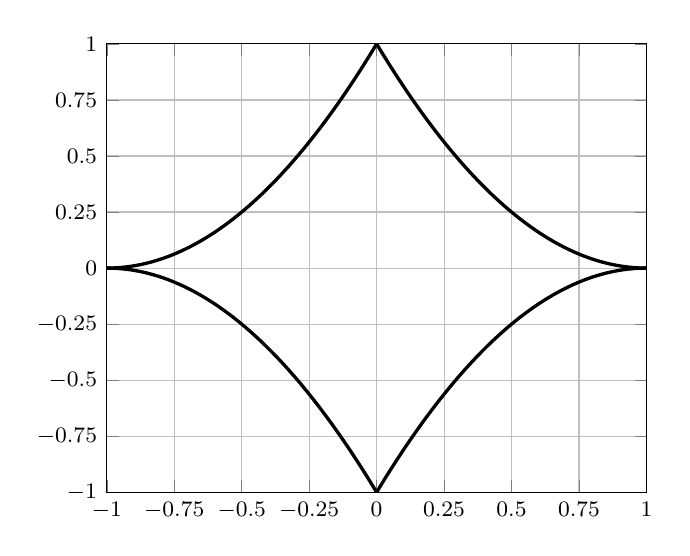
\begin{tikzpicture}
\begin{axis}[grid=major, xtick={-1,-0.75,...,1}, ytick={-1,-0.75,...,1}, xmin= -1, xmax=1, ymin=-1, ymax=1,tick label style={font=\footnotesize}]
\addplot[ very thick,samples=500] {(x-1)^2} ;
\addplot[ very thick,samples=500] {(-x-1)^2} ;
\addplot[ very thick,samples=500] {-(x-1)^2} ;
\addplot[ very thick,samples=500] {-(-x-1)^2} ;
\end{axis}
\end{tikzpicture}
\end{center}
  \item Use change of variables to derive a closed-form expression for the function
 \begin{align}
f(t) := \int_{0}^{t} \frac{x}{1+x^2} \diff{x}.
 \end{align}
\end{enumerate}

%\item (Gradients)
%Recall that the entries of the gradient of a function are equal to its partial derivatives. Use this fact to: 
%\begin{enumerate}
%\item Compute the gradient of $f(x) = b^T x$ where $b \in \R^{d}$ and $f: \R^{d} \rightarrow \R $.
%\item Compute the gradient of $f(x) = x^T A x$ where $A \in \R^{d\times d}$ and $f: \R^{d} \rightarrow \R $.
%\end{enumerate}
  
\end{enumerate}
\end{document}
